\documentclass[twocolumn]{aastex631}
\received{\today}
\shorttitle{LEGWORK}
\graphicspath{{./}{figures/}}

\usepackage{physics}
\usepackage{mathtools}
\usepackage{etoolbox}

% remove indents in footnotes
\usepackage[hang,flushmargin]{footmisc} 

\newcommand{\todo}[1]{{\color{red}{[TODO: #1}]}}

% custom function for adding units
\makeatletter
\newcommand{\unit}[1]{%
    \,\mathrm{#1}\checknextarg}
\newcommand{\checknextarg}{\@ifnextchar\bgroup{\gobblenextarg}{}}
\newcommand{\gobblenextarg}[1]{\,\mathrm{#1}\@ifnextchar\bgroup{\gobblenextarg}{}}
\makeatother

\newcommand{\avg}[1]{\left\langle#1\right\rangle}

% define colour from xcolor
\definecolor{SeaGreen}{RGB}{63, 188, 157}

% LEGWORK stuff
\newcommand{\lw}{LEGWORK}
\newcommand{\lwColour}{SeaGreen}
\newcommand{\lwModURL}[1]{https://legwork.readthedocs.io/en/latest/modules.html\#module-legwork.#1}
\newcommand{\lwModLink}[1]{\href{https://legwork.readthedocs.io/en/latest/modules.html\#module-legwork.#1}{\color{\lwColour}{\texttt{#1}}}}
\newcommand{\lwFuncURL}[2]{https://legwork.readthedocs.io/en/latest/api/legwork.#1.#2.html\#legwork.#1.#2}

% icons and links
\newcommand{\docsIcon}{{\color{\lwColour}{\faFileCode}}}
\newcommand{\docsLink}[1]{\href{#1}{\docsIcon}}

\newcommand{\tutorialIcon}{{\color{\lwColour}{\faLaptopCode}}}
\newcommand{\tutorialLink}[1]{\href{#1}{\tutorialIcon}}

% add documentation links to equation environments
% Luger+19 inspired this!
\newtagform{eqtag}[]{(}{)}

\renewenvironment{equation}[1]{%
    \ifstrempty{#1}{%
        \renewtagform{eqtag}[]{(}{)}%
    }{%
        \renewtagform{eqtag}[]{\docsLink{#1}\,(}{)}%
    }%
    \usetagform{eqtag}%
    \align%
    }{%
    \endalign%
    \renewtagform{eqtag}[]{(}{)}%
    \usetagform{eqtag}%
}

\begin{document}

\title{LEGWORK: LISA Evolution and Gravitational Wave Orbit Kit}

% affiliations
\newcommand{\cfa}{Center for Astrophysics | Harvard \& Smithsonian, 60 Garden Street, Cambridge, MA 02138, USA}
\newcommand{\mpa}{Max-Planck-Institut für Astrophysik, Karl-Schwarzschild-Straße 1, 85741 Garching, Germany}
\newcommand{\cca}{Center for Computational Astrophysics, Flatiron Institute, 162 Fifth Ave, New York, NY, 10010, USA}
\newcommand{\UoA}{Anton Pannekoek Institute for Astronomy and GRAPPA, University of Amsterdam, NL-1090 GE Amsterdam, The Netherlands}
\newcommand{\UW}{Department of Astronomy, University of Washington, Seattle, WA, 98195}

\author[0000-0001-6147-5761]{T. Wagg}
\affiliation{\UW}
\affiliation{\cfa}
\affiliation{\mpa}

\author[0000-0001-5228-6598]{K. Breivik}
\affiliation{\cca}

\author[0000-0001-9336-2825]{S. E. de Mink}
\affiliation{\mpa}
\affiliation{\UoA}
\affiliation{\cfa}

\correspondingauthor{Tom Wagg}
\email{tomjwagg@gmail.com}

\begin{abstract}
    We present \lw{}, a Python package for making predictions about stellar-origin gravitational wave sources and their detectability in LISA and other space-based gravitational wave detectors. \lw{} can be used to evolve sources over time, calculate gravitational wave strains, compute signal-to-noise ratios and visualise the results. In this paper we give an overview of the structure and functionality of the package, as well as highlight several optimisations that make it particularly efficient. We demonstrate the various capabilities of \lw{} through a series of example use cases. These begin with a basic example of calculating the signal-to-noise ratio of a source but also include using \lw{} to calculate horizon distances and make comparisons between gravitational-wave detectors. We additionally explain in detail the derivation of the equations behind \lw{} in order to clarify some conflicts currently present in the literature.
\end{abstract}

\keywords{gravitational waves, LISA}

\section{Introduction}

The planned space-based gravitational wave detector LISA (Laser Interferometer Space Antenna) will present an entirely new view of gravitational waves by focusing on lower frequencies ($10^{-5} < f / \unit{Hz} < 10^{-1}$) than ground-based detectors. This will enable the study of the gravitational wave mergers of supermassive black holes that are undetectable with ground-based detectors \citep[e.g.][]{Begelman+1980, Klein+2016}. However, this frequency regime is also of interest for the detection of local stellar-mass binaries during their inspiral phase. LISA is expected to detect Galactic stellar-origin compact objects, ranging from the numerous double white dwarf (WDWD) population, to the rare but loud double black hole (BHBH) population.

The potential to detect stellar-origin sources with LISA has been studied in the past \citep[e.g.][]{Nelemans+2001, Belczynski+2010}. More recently, the direct detection of gravitational waves with ground-based detectors has led to renewed interest in this topic with many recent papers addressing the issue \citep[e.g.][]{Christian+2017, Kremer+2017, Kremer+2018, Korol+2017, Korol+2018, Korol+2019, Korol+2020, Lamberts+2018, Lamberts+2019, Fang+2019, Andrews+2020, Lau+2020, Breivik+2020, Breivik+2020a, Roebber+2020, Chen+2020, Sesana+2020}.

Each of these studies require making estimates of the signal-to-noise ratio of individual binary systems and possibly the slow gravitational wave inspiral that lead to the present-day parameters. So far, most studies made use of custom made codes which have not been made publicly available. 

We believe that the large renewed interest in LISA and the stellar-origin sources it may detect will lead to many more studies in the near future that would need similar computations. This leads to a significant amount of redundancy which, at best results in extra work for each individual and at worst leads to an increased chance of introducing mistakes and inconsistencies when coding up the necessary expressions.

\lw{} is a Python package designed to streamline the process of making predictions of LISA detection rates for stellar-origin binaries such that it is fast, reliable and simple. With \lw{} one can evolve the orbits of a binary or a collection of binaries and calculate their strain amplitudes for any range of harmonics. One can compute the sensitivity curve for LISA or other future gravitational wave detectors (e.g. TianQin's curve, or that of a custom instrument) and use it to compute the signal-to-noise ratio of a collection of sources. Furthermore, \lw{} provides tools to visualise all of the results with easy-to-use plotting functions.

Specifically, we implement the expressions by \citet{Peters+1963} and \citet{Peters+1964} for the evolution of binary orbits, equations for the strain amplitudes and signal-to-noise ratios of binaries from various papers \citep[e.g.][]{Flanagan+1998, Finn+2000, Barack+2004, Moore+2015} and approximations for the LISA and TianQin sensitivity curves given in \citet{Robson+2019} and \citet{Huang+2020} respectively.

The open-source nature of the project means that new users as well as seasoned experts in the field can work together in a collaborative setting to consider new features and enhancements to the package as well as check the implementation. At the same time, with our thorough online documentation, derivations and tutorials, we hope \lw{} can make this functionality more accessible to the broader scientific community.

\lw{} can be installed with pip or obtained from the GitHub repository \href{https://github.com/TeamLEGWORK/LEGWORK}{\faGithub}\footnote{\url{https://github.com/TeamLEGWORK/LEGWORK}}. All examples shown in this paper and code to reproduce the figures are available in the repository. Instructions for installation and basic usage are provided in the online documentation\footnote{\url{https://legwork.readthedocs.io/en/latest/}} which contain the most up-to-date instructions.

The paper is organised as follows. In Section~\ref{sec:LEGWORK-overview} we give an overview of the capabilities of the \lw{} package and its various modules. In Section~\ref{sec:example-uses} we outline some example use cases of \lw{} to demonstrate its use. We detail the derivations of the equations relevant for \lw{} in Section~\ref{sec:derivations}. Finally, in Section~\ref{sec:summary} we conclude and summarise our work.

\section{Package Overview}\label{sec:LEGWORK-overview}

\begin{figure}
    \centering
    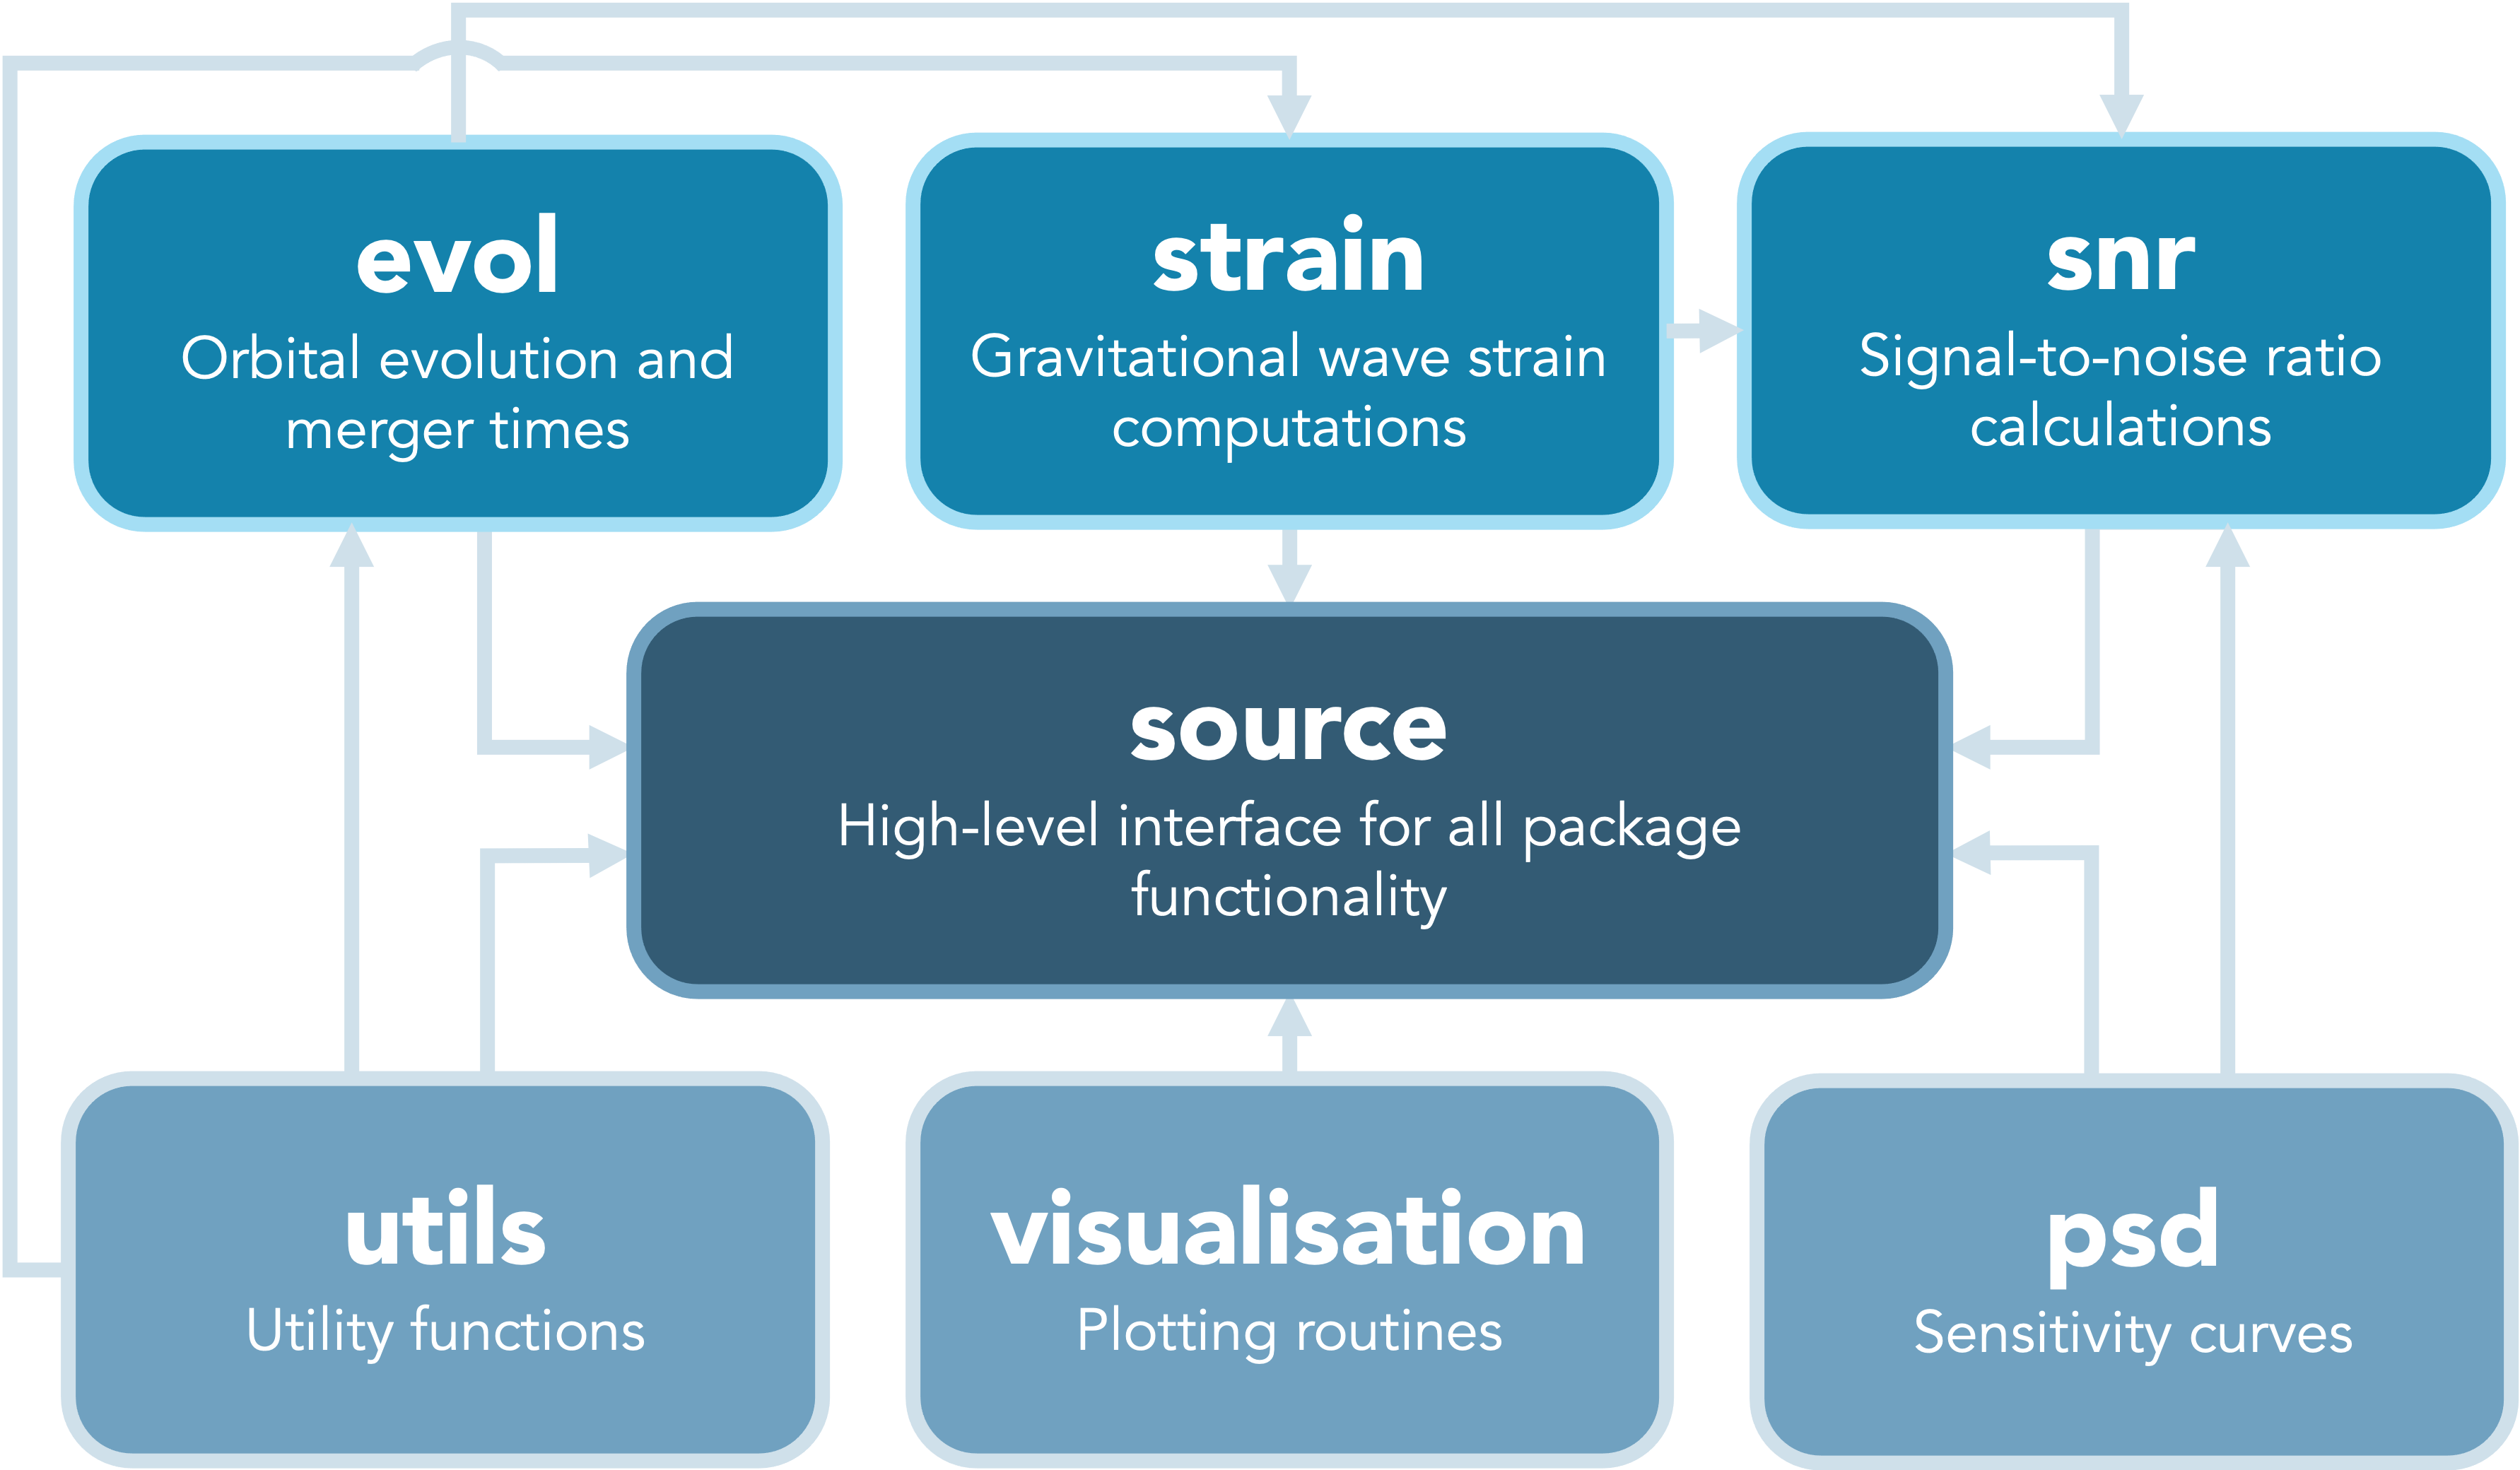
\includegraphics[width=\columnwidth]{static/package_overview.png}
    \caption{Package structure of \lw{}. Each box represents a module and describes its function. The arrows indicate the inter-dependencies of the modules.}
    \label{fig:package_overview}
\end{figure}

The \lw{} package is composed of seven modules that each focus on a particular aspect of calculations useful for LISA gravitational wave sources. In Fig.~\ref{fig:package_overview}, we illustrate the general structure of the package with its various modules. The source module is the central module of the package and provides an simple interface to the functions in the rest of the modules. For more complex analyses, users may want to interact directly with individual modules, particularly those in the top row of Fig.~\ref{fig:package_overview} as they comprise the core functionality of \lw{}. Below we explain the capabilities of each module in detail.

\lwModLink{evol} deals with the orbital evolution of a binary due to gravitational waves. It includes functions for computing the merger times of both circular and eccentric binaries. In addition, you can use this module to evolve binary orbit parameters forward in time with any number or arrangement of timesteps. We discuss the relevant equations in Sec.~\ref{sec:deriv_evol}.

\lwModLink{strain} contains two functions that compute a binary's gravitational wave strain and characteristic strain amplitude respectively. Each of these functions is capable of computing the strain for a 3-dimensional array of binaries at any number of timesteps and evaluated at any number of harmonics. We discuss the relevant equations in Sec.~\ref{sec:deriv_strain}.

\lwModLink{psd} is used for evaluating the effective noise power spectral density of a detector at different frequencies. The module contains both the LISA and TianQin sensitivity curves that can be tweaked by adjusting parameters such as the observation time, confusion noise and even the arm length. Additionally, this module allows the user to specify a custom detector sensitivity curve. We discuss the relevant equations in Sec.~\ref{sec:deriv_psd}.

\lwModLink{snr} uses the functions in \texttt{evol}, \texttt{strain} and \texttt{psd} to compute the signal-to-noise ratio of sources. It contains four functions that cover the permutations of whether a source is circular or eccentric and stationary in frequency space on the timescale of the mission or evolving. We discuss the relevant equations in Sec.~\ref{sec:deriv_snr}.

\lwModLink{visualisation} contains several wrappers for plotting 1- and 2-dimensional distributions with histograms, scatter plots, and kernel density estimator (KDE) plots in order to quickly analyse a collection of sources. In addition, it provides functions for plotting sources directly onto a sensitivity curve.

\lwModLink{source} provides a direct and simple interface to the functions in other modules through the \texttt{Source} Class. You can instantiate this Class with an array of sources and use it compute their strains or signal-to-noise ratios directly. Moreover, depending on the user's choice of allowed gravitational wave luminosity error, the Class dynamically decides on the number of harmonics needed to capture the full signal of each binary and at what eccentricity to no longer consider a binary circular. This Class also provides a quick means of evolving the sources, visualising the parameters of each source and allows you to plot the binaries on the sensitivity curve.

\lwModLink{utils} is a collection of miscellaneous utility functions mainly consisting of conversions between variables as well as constants and expressions from \citet{Peters+1964}. We discuss the relevant equations in Sec.~\ref{sec:deriv_utils}.

\subsection{Optimistations}

We developed \lw{} with an emphasis on increasing the efficiency of these computations in order to make large scale simulations more tractable. As a simple first step, we ensured that the entirety of \lw{} is vectorised and thus scales well with larger populations. In addition, we made a several specific optimisations to further increase the speed of calculations.

In certain cases one can apply approximations in place of the general SNR calculations. Although it is possible to use each of these approximations directly through the \lwModLink{snr} module, the \lwModLink{source} module will automatically apply the most appropriate function for each individual source. \lw{} dynamically classifies each source as one of four types, which cover the permutations of whether a binary is effectively circular or eccentric and whether or not it is stationary in frequency space on the timescale of the LISA mission. Then when computing the SNR, it applies a different function to each type of the source. This avoids computing unnecessary, time intensive integrals.

Moreover, for increasingly eccentric sources, gravitational waves are emitted in an increasing number of higher harmonics. Although the total SNR is formally calculated as a the sum of the SNR over an infinite number of harmonics, in practice it is sufficient to only consider a subset. In the \lwModLink{source} module, the user can provide \texttt{gw\_lum\_tol}, a maximum allowable tolerance for the accuracy of the gravitational wave luminosity. Given this tolerance, \lw{} automatically calculates the required number of harmonics to satisfy this tolerance and thus minimise the computation time.

Lastly, as a simple (yet thoroughly effective) optimisation, we interpolate (1) $g(n, e)$, which is a complicated combination of Bessel functions used in several calculations (see Eq.~\ref{eq:g(n,e)}) (2) the given sensitivity curve $S_{\rm n}(f)$. This significantly reduces the runtime of most strain and SNR calculations for large populations of sources.

\section{Use cases}\label{sec:example-uses}
In this section, we demonstrate \lw{}'s range of capabilities through a series of example use cases. The plots and results in each subsection are reproduced directly in online demos in the \lw{} documentation, which are each based on individual Jupyter notebooks. These tutorials are linked at the start of each subsection with the \tutorialIcon{} icon.

\subsection{Computing the SNR of a binary system\texorpdfstring{ - \tutorialLink{https://legwork.readthedocs.io/en/latest/demos/BasicSNRCalculation.html}}{}}

The most fundamental use case of \lw{} is to compute the SNR of a binary system in LISA. This can be accomplished in \lw{} with only two lines of code - one line to set up the source and another to compute the SNR. As an example one could consider a binary with the parameters
\begin{align*}
    m_1 = m_2 &= 10 \unit{M_{\odot}},\ d = 8 \unit{kpc},\\
    f_{\rm orb} &= 10^{-4} \unit{Hz},\ e = 0.2,
\end{align*}
where $m_1, m_2$ are the primary and secondary masses, $d$ is the distance to the source, $f_{\rm orb}$ is the orbital frequency and $e$ is the eccentricity. As we don't specify a position, polarisation or inclination, \lw{} will calculate the SNR averaged over these quantities. One can now instantiate a source in \lw{} using these parameters (leaving the LISA mission parameters as the default values, such that we compute the SNR for a 4-year LISA mission). As shown in the linked demo, \lw{} quickly computes that the SNR of this binary is $4.49$. In the background, \lw{} decides which SNR approximation is most applicable given the eccentricity of the binary and whether it is stationary in frequency space.

Moreover, this can be generalised to a population of many binary systems with ease. Instead of inputting single values for each parameter, one can input arrays of values where each entry corresponds to a different binary. As an example, we can take the same parameters as above for 3 different binaries but vary the primary as $m_1 = [5, 10, 15] \unit{M_{\odot}}$. Using \lw{} we find that the SNR for each of these cases is $\rho = [2.47, 4.49, 7.85]$.

\subsection{Horizon distance\texorpdfstring{ - \tutorialLink{https://legwork.readthedocs.io/en/latest/demos/HorizonDistance.html}}{}}

\begin{figure*}[htb]
    \centering
    \includegraphics[width=\textwidth]{figures/horizon_distance.pdf}
    \caption{The horizon distance for circular stellar mass binaries in a four-year LISA mission. The filled contours indicate the horizon distance for different orbital frequencies and chirp masses. We add white dotted contours at $8, 50, 800 \unit{kpc}$ and $40 \unit{Mpc}$ to highlight the distances to the centre of the Milky Way, the Magellanic Clouds, the Andromeda galaxy and the nearest ground-based gravitational wave detection (GW170817, \citealp{Abbott+2017_GW170817}) respectively. The diagonal line black line shows the frequencies and chirp masses at which the merger time is equal to the observation time. This line emphasises the sharp contrast for the horizon distance for binaries that merge before the LISA mission finishes observing (to the right of the line). The horizontal black lines indicate the approximate location of some common double compact object types on this plot, with the assumed masses labelled below in solar masses.}
    \label{fig:horizon_distance}
\end{figure*}

A common question to consider with stellar mass sources in LISA is how far away a certain source could be detected. In other words, what is the horizon distance beyond which a source no longer has a SNR greater than some chosen threshold. We can explore this question using \lw{}.

Let us compute the horizon distance for a grid of chirp masses and orbital frequencies. First, we can recall that the signal-to-noise ratio of a source is inversely proportional to its distance from LISA and so we can find the horizon distance, $D_{\rm hor}$ as
\begin{equation}{}
    \label{eq:snr_to_hor_dist}
    D_{\rm hor} = \frac{\rho(D)}{\rho_{\rm detect}} \cdot D,
\end{equation}
where $\rho(D)$ is the signal-to-noise ratio as some distance $D$ and $\rho_{\rm detect}$ is the threshold above which we consider a source to be detectable. For the purpose of this example we will set $\rho_{\rm detect} = 7$. Therefore, we can start by finding the signal-to-noise ratio for each source at an arbitrary distance and convert that to a horizon distance.

This can be most efficiently accomplished using \lw{}'s source class. Although the source class only takes one-dimensional lists of sources, one can flatten a grid of chirp masses and orbital frequencies to make the input work. \lw{} can then compute the merger times and signal-to-noise ratio of each source with only two lines of code. These results can then be reshaped to match the original grid of chirp masses and frequencies.

We convert these SNRs to horizon distances using Eq.~\ref{eq:snr_to_hor_dist} and plot the result in Figure~\ref{fig:horizon_distance}. The shape of the LISA sensitivity curve is clearly reflected in this plot of the horizon distance. This is because circular sources emit the vast majority of their single at a single frequency and thus every feature in the sensitivity curve has a strong effect on the SNR (and therefore horizon distance) for circular sources. We also see that once the merger time of a source is shorter than the LISA mission length (shown by the black dotted line), the horizon distance sharply decreases. This is because if a source merges before the LISA mission concludes, it has less time to accumulate signal and thus has a lower SNR and horizon distance.

One can use Figure~\ref{fig:horizon_distance} to estimate the horizon distance for any circular source of interest. To illustrate this, we add solid black lines to indicate the typical chirp masses of some possible stellar mass gravitational wave sources as well as white dotted lines to show the distances to nearby galaxies as well as the nearest ground-based gravitational wave detection (GW170817, \citealp{Abbott+2017_GW170817}). For example, we see that a circular NSNS with an orbital frequency greater than a mHz is detectable in the Magellanic clouds.

\subsection{The role of eccentricity\texorpdfstring{ - \tutorialLink{https://legwork.readthedocs.io/en/latest/demos/TheRoleofEccentricity.html}}{}}\label{sec:eccentricity_role}

The role of eccentricity is an important concept to consider in the detection of gravitational waves with LISA as sources can still have significant eccentricity during their inspiral phase. A high eccentricity has two major effects on the SNR of a gravitational wave source in LISA and we can investigate this using \lw{}.

Let's use three toy sources that are identical apart from their eccentricities, $e_i$.
\begin{align*}{}
    m_1 &= m_2 = 0.6 \unit{M_{\odot}}, f_{\rm orb} = 1.5 \unit{mHz}, d = 15 \unit{kpc}, \\
    e_i &= \{0.0, 0.6, 0.9 \},
\end{align*}
Using \lw{} to calculate their signal-to-noise ratios, $\rho_i$, we find
\begin{equation*}{}
    \rho_i = \{ 31.7, 50.2, 38.8 \}
\end{equation*}

We see two effects in the signal-to-noise ratio here. First, increasing the eccentricity from essentially circular to $e = 0.6$ results in a higher signal-to-noise ratio ($\rho=31.7 \to \rho=50.2$). This is because an eccentric binary has enhanced energy emission via gravitational waves \citep{Peters+1963}. This means that an eccentric binary will not only inspiral faster than an otherwise identical circular binary, but also will always have a stronger gravitational wave strain. The enhancement factor and its exact dependence on eccentricity is discussed in more detail Section~\ref{sec:derivations} (specifically Eq.~\ref{eq:eccentricity_enhancement_factor}).

The second effect is more intriguing. We see that increasing the eccentricity from $e = 0.6$ to $e = 0.9$ results in a relative \textit{decrease} in SNR ($\rho=50.2 \to \rho=38.8$). The reason for this is that eccentric binaries emit gravitational waves at many harmonic frequencies (unlike circular binaries, which emit predominantly twice the orbital frequency). This leads to the gravitational wave signal being diluted over many frequencies higher than the orbital frequency, where the higher the eccentricity, the more harmonics are required to capture all of the gravitational luminosity \citep[see][Fig.\,3]{Peters+1963}. Therefore, if the eccentricity is too high, the majority of the signal may be emitted at a frequency to which LISA is less sensitive.

We can illustrate this point with \lw{} by calculating the SNR at each individual harmonic using the \lwModLink{snr} module. We plot this distribution of signal over different harmonics with the LISA sensitivity curve overlaid in Fig.~\ref{fig:role_eccentricity} using \lw{}'s \lwModLink{visualisation} module. A point is plotted for each harmonic of each source that has an SNR greater than unity and such that its height above the sensitivity curve corresponds to its SNR.

\begin{figure}[tb]
    \centering
    \includegraphics[width=\columnwidth]{figures/role_eccentricity.pdf}
    \caption{An illustration of the effect of eccentricity on the detectability of a LISA source. The three sets of points are coloured by their eccentricity and each individual point corresponds to a harmonic frequency, where its height above the curve gives its SNR. We annotate each set of points with its total SNR and overlay the LISA sensitivity curve. The dotted vertical lines indicate the frequency at which the majority of the gravitational wave signal is concentrated.}
    \label{fig:role_eccentricity}
\end{figure}

From Fig.~\ref{fig:role_eccentricity}, we can better understand why a source with $e = 0.9$ has a lower SNR than the same source with $e = 0.6$. From the dotted lines, we can note that the signal from the $e = 0.9$ source is concentrated at a frequency of around $4 \times 10^{-2} \unit{Hz}$. The LISA sensitivity at this point is much weaker than the $6 \times 10^{-3} \unit{Hz}$ at which the $e =0.6$ source is concentrated. Therefore, although the strain from a more eccentric binary is stronger, the SNR is lower due to the increased noise in the LISA detector.

Overall, we can therefore conclude that for LISA sources of this nature, higher eccentricity will produce more detectable binaries only if the orbital frequency is not already at or above the minimum of the LISA sensitivity curve.

\begin{figure}[htb]
    \centering
    \includegraphics[width=\columnwidth]{figures/merger_time.pdf}
    \caption{The merger time for a binary with both a primary and secondary mass of $10 \unit{M_{\odot}}$ over different eccentricities and orbital frequencies.}
    \label{fig:merger_time}
\end{figure}

Another consideration for more massive binaries is whether the increased eccentricity will cause the binary to merge before the mission ends, which would cause a significant decrease in signal-to-noise ratio. We can also use \lw{} to find how the merger time of a source varies with frequency and eccentricity over a grid of sources.

We plot the results of this calculation in Figure~\ref{fig:merger_time}. This plot shows that for most eccentricities the merger is time is largely determined by the orbital frequency. However, for high eccentricities ($e > 0.8$), the eccentricity significantly reduces the merger time.

\subsection{Compare gravitational wave detectors\texorpdfstring{ - \tutorialLink{https://legwork.readthedocs.io/en/latest/demos/CompareSensitivityCurves.html}}{}}

It may also be useful to consider how changing the specifications of the LISA detector, or using a different detector entirely, could affect the SNR of a particular source. \lw{} is capable of adjusting the LISA mission specifications or using a different sensitivity curve and thus we can use it to explore these differences.

As a first step, we can use \lw{} to plot a series of sensitivity curves in Figure~\ref{fig:detector_sc_compare}. We show the LISA sensitivity curve for the default 4 year mission length but also illustrate how the curve changes for shorter mission lengths. At 0.5 and 2 years, we see a stronger noise level around $3 \unit{mHz}$ as a result of the increased Galactic confusion noise. This noise decreases with increasing mission length since more individual foreground sources can be resolved and thus removed from the confusion noise. We also see that using an approximated response function smooths out the sensitivity curve at higher frequencies. Finally, the TianQin curve is higher than the 4 year LISA curve until around $5 \unit{mHz}$, beyond which it has a lower noise level.

\begin{figure}[htb]
    \centering
    \includegraphics[width=\columnwidth]{figures/detector_sc_compare.pdf}
    \caption{The strain spectral density of the LISA detector (with different specifications) and the TianQin detector. We show the LISA curve for three different mission lengths and once with an approximate response function.}
    \label{fig:detector_sc_compare}
\end{figure}

Although comparing the sensitivity curves would suffice for a stationary and circular source (since it would remain at a single frequency), \lw{} can also be used to see how the relative SNR between two detectors changes over a range of eccentricities and frequencies.

Using \lw{}, we can compute the SNR of a grid of sources (spanning a range of frequencies and eccentricities) for both detectors. In Figure~\ref{fig:detector_snr_ratio}, we show the ratio of the SNR in LISA to the SNR in TianQin. This plot shows that for circular binaries, the SNR of the source in LISA is stronger up to an orbital frequency of approximately $2.5 \unit{mHz}$, beyond which the SNR of the source is stronger in TianQin. This transition frequency becomes lower with increasing eccentricity as one would expect since eccentric sources emit more at higher harmonics and thus higher frequencies.

\begin{figure}[htb]
    \centering
    \includegraphics[width=\columnwidth]{figures/detector_snr_ratio.pdf}
    \caption{The ratio of the SNR in LISA (for a four year mission) to the SNR in TianQin. The dashed line indicates the transition at which the SNR is equal in both detectors. We annotate the regions in which either detector has a higher SNR and also annotate the mass and distance of each source in the grid.}
    \label{fig:detector_snr_ratio}
\end{figure}

\subsection{Track SNR of a binary over time\texorpdfstring{ - \tutorialLink{https://legwork.readthedocs.io/en/latest/demos/SNROverTime.html}}{}}

As a binary inspirals its orbital frequency and eccentricity change and this in turn affects the SNR of the binary. For this use case we will demonstrate how \lw{} can be used to track the evolution of these parameters and pinpoint the moment at which a binary becomes detectable.

Let's consider a binary with the following initial parameters
\begin{align*}
    m_1 &= m_2 = 15 \unit{M_{\odot}},\ d = 20 \unit{kpc},\\
    f_{\rm orb, i} &= 3 \times 10^{-5} \unit{Hz},\ e_i = 0.5,
\end{align*}
and use \lw{} to evolve the system until 100 years before its merger with 1000 linearly spaced timesteps, recording the eccentricity and frequency at each timestep.

We plot this evolution of the eccentricity and frequency in the top two panels of Fig.~\ref{fig:snr_over_time} as a function of the time before the merger. We see that the binary circularises and increases its orbital frequency as it inspirals as we would expect.

To take this a step further, we can consider the binary at each timestep to be a separate source with the current eccentricity and frequency. It is then trivial to use \lw{} to calculate the SNR for each of these `sources' and thus attain the SNR evolution, which we plot in the last panel of Fig.~\ref{fig:snr_over_time}.

We see that the SNR increases monotonically over time and sharply increases as the binary approaches its merger. Around $1 \unit{Myr}$ before the merger, the SNR reaches the detection threshold and thus could then be seen by a 4-year LISA mission.

Note that \lw{} could also be used in this way to find the SNR of any system in which the orbital evolution is know. Thus for a triple system or a binary experiencing gas drag (as long the evolution of the eccentricity and orbital frequency is known) \lw{} is entirely capable of calculating the SNR evolution.

\begin{figure}
    \centering
    \includegraphics[width=\columnwidth]{figures/snr_over_time.pdf}
    \caption{The evolution of a binary system's eccentricity (top), orbital frequency (middle) and signal-to-noise ratio (bottom). Each panel is annotated with the constant parameters of the system. The SNR is calculated for a 4-year LISA mission. We annotate in  a line the bottom panel at $\mathrm{SNR} = 7$ to highlight the moment at which the source becomes detectable.}
    \label{fig:snr_over_time}
\end{figure}

% \subsection{SNR calculation for verification binaries}

%\section{Benchmarks}\label{sec:speed}
%A section to show off \lw{}'s speed.

\section{Derivations}\label{sec:derivations}
In this section, we present a derivation of the equations using in \lw{}. We emphasise that these are not new derivations, conversely, they are in fact given frequently in the literature. However, they are often incomplete, unclear or contain spurious constant factors that arise from invalid combinations of previous work. Here, we aim to present a clear, clean and concise explanation of the expressions we use in \lw{}.

A \docsIcon{} symbol in an equation will link to the relevant \lw{} documentation for the implementation of that equation. These derivations are also given in more detail in the \lw{} documentation \href{https://legwork.readthedocs.io/en/latest/notebooks/Derivations.html}{here}, where we show each of the intervening steps in more detail.

\subsection{Conversions and definitions {\normalfont (\texorpdfstring{\lwModLink{utils}}{utils})}}\label{sec:deriv_utils}
We start these derivations by defining some useful conversions and definitions. The chirp mass of a binary is the mass quantity measured by LISA and is given by
\begin{equation}{\lwFuncURL{utils}{chirp_mass}}
    \mathcal{M}_c \equiv \frac{(m_1 m_2)^{3/5}}{(m_1 + m_2)^{1/5}},
    \label{eq:chirpmass}
\end{equation}
where $m_1$ and $m_2$ are the primary and secondary masses of the double compact object. 

It is often convenient to convert between orbital frequency, $f_{\rm orb}$, and the semi-major axis, $a$, of a binary and this can be accomplished with Kepler's third law.
\begin{equation}{\lwFuncURL{utils}{get_a_from_f_orb}}
    a = \qty(\frac{G(m_1 + m_2)}{(2 \pi f_{\rm orb})^{2}})^{1/3},
    \label{eq:kepler3rd}
\end{equation}
or inversely
\begin{equation}{\lwFuncURL{utils}{get_a_from_f_orb}}
    f_{\rm orb} = \frac{1}{2 \pi} \sqrt{\frac{G(m_1 + m_2)}{a^3}}.
    \label{eq:kepler3rd_reverse}
\end{equation}

For eccentric binaries, we need to consider all harmonics of gravitational wave emission. These are defined such that the $n^{\rm th}$ harmonic frequency is
\begin{equation}{}
    f_{n} \equiv n \cdot f_{\rm orb}.
    \label{eq:nth_freq}
\end{equation}
It will be important to know the relative power radiated into the $n^{\rm th}$ harmonic for a binary with eccentricity $e$, which is given by \citep[][Eq.\,20]{Peters+1963}
\begin{equation}{\lwFuncURL{utils}{peters_g}}
    \begin{aligned}
        g(n, e) = \frac{n^{4}}{32} & \Big\{ \Big[ J_{n-2}(n e)-2 e J_{n-1}(n e)+\frac{2}{n} J_{n}(n e) \\
        &\left. +2 e J_{n+1}(n e)-J_{n+2}(n e)\Big]^{2}\right.\\
        &\left.\kern-\nulldelimiterspace\right.
            \!\!\begin{aligned}
            +\big(1-e^{2}\big)\Big[&J_{n-2}(n e)-2 J_{n}(n e) \\
            &+J_{n+2}(n e)\Big]^{2} \\
            \end{aligned}\\
        &+\frac{4}{3 n^{2}}\Big[J_{n}(n e)\Big]^{2}\Big\},
    \end{aligned}
    \label{eq:g(n,e)}
\end{equation}
where $J_{n}(v)$ is the Bessel function of the first kind. Thus, the \textit{sum} of $g(n, e)$ over all harmonics gives the factor by which the gravitational wave emission is stronger for a binary of eccentricity $e$ over an equivalent circular binary. This enhancement factor is \citep[][Eq.\,17]{Peters+1963}
\begin{equation}{\lwFuncURL{utils}{peters_f}}
    F(e) \equiv \sum_{n = 1}^{\infty} g(n, e) = \frac{1 + \frac{73}{24} e^2 + \frac{37}{96} e^4}{(1 - e^2)^{7/2}}.
    \label{eq:eccentricity_enhancement_factor}
\end{equation}
A fun number to remember is that $F(0.5) \approx 5.0$, or in words, a binary with eccentricity $0.5$ loses energy to gravitational waves at 5 times the rate of an equivalent circular binary.

\subsection{Orbital evolution {\normalfont (\texorpdfstring{\lwModLink{evol}}{evol})}}\label{sec:deriv_evol}
\subsubsection{Circular binaries}
For a circular binary, the evolution can be calculated analytically, as the rate at which the separation of the binary shrinks is simply a function of its mass and the current separation \citep[][Eq.~5.6]{Peters+1964}
\begin{equation}{}
    \dv{a}{t}_{e = 0} = -\frac{\beta}{a^3},
\end{equation}
where the constant $\beta$ is defined as
\begin{equation}{\lwFuncURL{utils}{beta}}
    \beta(m_1, m_2) = \frac{64}{5} \frac{G^3}{c^5} m_1 m_2 (m_1 + m_2),
    \label{eq:beta_peters}
\end{equation}
where $m_1$ is the primary mass and $m_2$ is the secondary mass. This gives the semi-major axis of a circular binary as a function of time, $t$, as \citep[][Eq.~5.9]{Peters+1964}
\begin{equation}{\lwFuncURL{evol}{evol_circ}}
    a(t, m_1, m_2) = [a_0^4 - 4 t \beta(m_1, m_2)]^{1/4},
    \label{eq:a_over_time_circ}
\end{equation}
where $a_0$ is the initial semi-major axis. Moreover, we can solve for the merger time, the time until the binary will merge, by setting the final semi-major axis in Eq.~\ref{eq:a_over_time_circ}
\begin{equation}{\lwFuncURL{evol}{get_t_merge_circ}}
    t_{\rm merge, circ} = \frac{a_0^4}{4 \beta}.
    \label{eq:t_merge_circular}
\end{equation}

\subsubsection{Eccentric binaries}
The orbital evolution is more complex for eccentric binaries since the semi-major axis and eccentricity both evolve simultaneously and depend on one another. These equations cannot be solved analytically and require numerical integration. The semi major axis, $a$, and eccentricity, $e$, are related as \citep[][Eq.~5.11]{Peters+1964}
\begin{equation}{\lwFuncURL{utils}{get_a_from_ecc}}
    a(e) = c_0 \frac{e^{12/19}}{(1 - e^2)} \left(1 + \frac{121}{304} e^2\right)^{870/2299},
    \label{eq:a_from_e}
\end{equation}
where $c_0$ satisfies the initial conditions such that $a(e_0) = a_0$. The time derivative of the eccentricity, $e$, is given by
\begin{equation}{\lwFuncURL{evol}{de_dt}}
    \frac{\mathrm{d}e}{\mathrm{d}t} = -\frac{19}{12} \frac{\beta}{c_{0}^{4}} \frac{e^{-29 / 19}\left(1-e^{2}\right)^{3 / 2}}{\left[1+(121 / 304) e^{2}\right]^{\frac{1181}{2299}}},
    \label{eq:dedt}
\end{equation}
which we can integrate to find $e(t)$ and convert to $a(t)$ using Eq.~\ref{eq:a_from_e} (\docsLink{\lwFuncURL{evol}{evol_ecc}}).

Inverting this function and applying the fact that we know that $e \to 0$ when the binary merges gives the merger time \citep[][Eq.~5.14]{Peters+1964}
\begin{equation}{\lwFuncURL{evol}{get_t_merge_ecc}}
    t_{\rm merge} = \frac{12}{19} \frac{c_{0}^{4}}{\beta} \int_0^{e_0} \frac{\left[1+(121 / 304) e^{2}\right]^{\frac{1181}{2299}}}{e^{-29 / 19}\left(1-e^{2}\right)^{3 / 2}} \mathrm{d}e.
    \label{eq:t_merge_eccentric}
\end{equation}
For very small or very large eccentricities we approximate this integral using the following expressions (given in unlabelled equations after \citealp[][Eq.~5.14]{Peters+1964})
\begin{align}
    t_{\rm merge,\, e^2 \ll 1} &= \frac{c_0^4}{4 \beta} \cdot e_0^{48 / 19}, \\
    t_{\rm merge,\, (1 - e^2) \ll 1} &= \frac{768}{425} \frac{a_0^4}{4 \beta} (1 - e_0^2)^{7/2}.
\end{align}

\subsection{Strains {\normalfont (\texorpdfstring{\lwModLink{strain}}{strain})}}\label{sec:deriv_strain}
The strength of a gravitational wave in a detector at any one moment is determined by the strain amplitude, $h_0$. However, for the LISA mission, the signal can be present in the detector for many years. This means that, the $n^{\rm th}$ harmonic of the binary will spend approximately $f_n / \dot{f}_n$ seconds (or $f_n^2 / \dot{f}_n$ cycles) in the vicinity of a frequency $f_n$ \citep{Finn+2000}. This leads to the signal `accumulating' at the frequency $f_n$.

Therefore, to account for the integration of the signal over the mission, we can introduce the `characteristic' strain amplitude of the $n^{\rm th}$ harmonic \citep[e.g][]{Finn+2000, Moore+2015}\footnote{Note that this is factor of 2 different from \citet{Finn+2000}. This is because the factor of 2 is already included in the \citet{Robson+2019} sensitivity curve and so we remove it here.}
\begin{equation}{}
    h_{c, n}^2 = \qty(\frac{f_n^2}{\dot{f}_n}) h_{0, n}^2,
    \label{eq:strain-charstrain}
\end{equation}
where $h_{0, n}$ is the strain amplitude in the $n^{\rm th}$ harmonic.

The characteristic strain represents the strain measured by the detector over the duration of the mission (approximated as a single broad-band burst), whilst the strain amplitude is the strength of the GW emission at each instantaneous moment.

\subsubsection{Characteristic Strain}

The characteristic strain from a stellar mass binary in the $n^{\rm th}$ harmonic is given by (e.g. \citealp[][Eq.\,56]{Barack+2004}; \citealp[][Eq.\,5.1]{ Flanagan+1998})
\begin{equation}{}
    h_{c,n}^2 = \frac{1}{(\pi D_L)^2} \qty( \frac{2 G}{c^3} \frac{\dot{E_n}}{\dot{f_n}} ),
    \label{eq:char_strain_dedf}
\end{equation}
where $D_L$ is the luminosity distance to the binary, $\dot{E}_n$ is the power radiated in the $n^{\rm th}$ harmonic and $\dot{f}_n$ is the rate of change of the $n^{\rm th}$ harmonic frequency.

The power radiated in the $n^{\rm th}$ harmonic can be expressed as \citep[][Eq. 19]{Peters+1963}
\begin{equation}{}
    \dot{E}_n = \frac{32}{5} \frac{G^{4}}{c^5} \frac{m_{1}^{2} m_{2}^{2}\left(m_{1}+m_{2}\right)}{a^{5}} g(n, e),
    \label{eq:edot_peters}
\end{equation}
where $g(n, e)$ is given in Eq.~\ref{eq:g(n,e)}. By substituting $a$ for $f_{\rm orb}$ (Eq.~\ref{eq:kepler3rd_reverse}) and applying the definition of the chirp mass (Eq.~\ref{eq:chirpmass}) we obtain a more useful form for making gravitational wave predictions
\begin{equation}{}
    \dot{E}_n(\mathcal{M}_c, f_{\rm orb}, e) = \frac{32}{5} \frac{G^{7 / 3}}{c^{5}}\left(2 \pi f_{\mathrm{orb}} \mathcal{M}_{c}\right)^{10 / 3} g(n, e). \label{eq:edot}
\end{equation}
The last term needed to define the characteristic strain in Eq.~\ref{eq:char_strain_dedf} is the rate of change of the $n^{\rm th}$ harmonic frequency as a result of gravitational wave inspiral, which we can write as
\begin{equation}{}
    \dot{f}_{n} = \dv{f_{n}}{a} \dv{a}{t}.
    \label{eq:fdot_chainrule}
\end{equation}
We can find an expression for $\dd{f_{n}} / \dd{a}$ by substituting Eq.~\ref{eq:kepler3rd_reverse} into Eq.~\ref{eq:nth_freq} and differentiating 
\begin{equation}{}
    \dv{f_{n}}{a} = -\frac{3 n}{4 \pi} \frac{\sqrt{G(m_1 + m_2)}}{a^{5/2}}.
    \label{eq:dfda}
\end{equation}
The rate at which the semi-major axis decreases is \citep[][Eq. 5.6]{Peters+1964}
\begin{equation}{}
    \dv{a}{t} = -\frac{64}{5} \frac{G^{3} m_{1} m_{2}\left(m_{1}+m_{2}\right)}{c^{5} a^{3}} F(e).
    \label{eq:dadt}
\end{equation}
Substituting Eq.~\ref{eq:dfda} and Eq.~\ref{eq:dadt} into Eq.~\ref{eq:fdot_chainrule} gives an expression for $\dot{f}_{n}$
\begin{equation}{}
    \dot{f}_n = \frac{48 n}{5 \pi} \frac{G^{7/2}}{c^5} \qty(m_1 m_2 (m_1 + m_2)^{3/2}) \frac{F(e)}{a^{11/2}},
\end{equation}
which, as above with $\dot{E}_n$, we can recast using Kepler's third law and the definition of the chirp mass
\begin{equation}{\lwFuncURL{utils}{fn_dot}}
    \dot{f}_n = \frac{48 n}{5 \pi} \frac{\qty(G \mathcal{M}_c)^{5/3}}{c^5} (2 \pi f_{\rm orb})^{11/3} F(e).
    \label{eq:fdot}
\end{equation}
With definitions of both $\dot{E}_n$ and $\dot{f}_n$, we are now in a position to find an expression for the characteristic strain by plugging Eq.~\ref{eq:edot} and Eq.~\ref{eq:fdot} into Eq.~\ref{eq:char_strain}:
\begin{equation}{\lwFuncURL{strain}{h_c_n}}
    h_{c,n}^2 = \frac{2^{5/3}}{3 \pi^{4/3}} \frac{(G \mathcal{M}_c)^{5/3}}{c^3 D_L^2} \frac{1}{f_{\rm orb}^{1/3}} \frac{g(n, e)}{n F(e)}. \label{eq:char_strain}
\end{equation}

\subsubsection{Strain}
In order to get an expression for the strain amplitude of gravitational waves in the $n^{\rm th}$ harmonic, we can use Eq.~\ref{eq:strain-charstrain} and plug in Eq.~\ref{eq:fdot} and Eq.~\ref{eq:char_strain} 
\begin{equation}{\lwFuncURL{strain}{h_0_n}}
    h_n^2 = \frac{2^{28/3}}{5} \frac{(G \mathcal{M}_c)^{10/3}}{c^8 D_L^2} \frac{g(n, e)}{n^2} \qty(\pi f_{\rm orb})^{4/3} . 
    \label{eq:strain}
\end{equation}

\subsection{Sensitivity Curves {\normalfont (\texorpdfstring{\lwModLink{psd}}{psd})}}\label{sec:deriv_psd}

\subsubsection{LISA}
For the LISA sensitivity curve we use the equations from \citet{Robson+2019}. The \textit{effective} strain spectral density of the noise is defined as
\begin{equation}{\lwFuncURL{psd}{lisa_psd}}
    S_{\rm n}(f) \equiv \frac{P_n(f)}{\mathcal{R}(f)} + S_c(f),
\end{equation}
where $P_{\rm n}(f)$ is the power spectral density of the detector noise and $\mathcal{R}(f)$ is the sky and polarisation averaged signal response function of the instrument. Alternatively if we expand out $P_n(f)$, approximate $\mathcal{R}(f)$ and simplify we find \citep[][Eq.~1]{Robson+2019}
\begin{equation}{}
    \begin{split}
        S_{\rm n}(f) &= \frac{10}{3 L^2} \qty(P_{\rm OMS}(f) + \frac{4 P_{\rm acc}(f)}{(2 \pi f)^4}) \\
        &\times \qty(1 + \frac{6}{10} \qty(\frac{f}{f_*}^2)) + S_c(f),
    \end{split}
    \label{eq:LISA_Sn}
\end{equation}
where $L = 2.5 \unit{Gm}$ is detector arm length, $f^* = c / 2 \pi L = 19.09 \unit{mHz}$ is the transfer frequency, 
\begin{equation}{}
    \begin{split}
        P_{\rm OMS}(f) &= \left(1.5 \times 10^{-11} \mathrm{m}\right)^{2} \\
        &\times \left(1+\left(\frac{2 \mathrm{mHz}}{f}\right)^{4}\right) \mathrm{Hz}^{-1},
    \end{split}
\end{equation}
is the single-link optical metrology noise \citep[][Eq.~10]{Robson+2019},
\begin{equation}{}
    \begin{split}
        P_{\rm acc}(f) &= \left(3 \times 10^{-15} \mathrm{ms}^{-2}\right)^{2}\left(1+\left[\frac{0.4 \mathrm{mHz}}{f}\right]^{2}\right)\\
        &\times \left(1+\left[\frac{f}{8 \mathrm{mHz}}\right]^{4}\right) \mathrm{Hz}^{-1},
    \end{split}
\end{equation}
is the single test mass acceleration noise \citep[][Eq.~11]{Robson+2019} and
\begin{equation}{}
    \begin{split}
        S_{c}(f)&=A f^{-7 / 3} e^{-f^{\alpha}+\beta f \sin (\kappa f)} \\
        &\times \left[1+\tanh \left(\gamma\left(f_{k}-f\right)\right)\right] \mathrm{Hz}^{-1},
    \end{split}
\end{equation}
is the galactic confusion noise \citep[][Eq.~14]{Robson+2019}, where the amplitude $A$ is fixed as $9 \times 10^{-45}$ and the various parameters change over time:
$$
    \begin{array}{|c|c|c|c|c|}
        \hline
        & 6 \mathrm{mo} & 1 \mathrm{yr} & 2 \mathrm{yr} & 4 \mathrm{yr} \\
        \hline
        \alpha & 0.133 & 0.171 & 0.165 & 0.138 \\
        \beta & 243 & 292 & 299 & -221 \\
        \kappa & 482 & 1020 & 611 & 521 \\
        \gamma & 917 & 1680 & 1340 & 1680 \\
        f_{k} & 0.00258 & 0.00215 & 0.00173 & 0.00113 \\
        \hline
    \end{array}
$$

\subsubsection{TianQin}
For the TianQin sensitivity curve we use the power spectral density given in \citet[][Eq.~13]{Huang+2020}
\begin{equation}{}
    \begin{split}
    S_{N}(f) &= \frac{1}{L^{2}}\left[\frac{4 S_{a}}{(2 \pi f)^{4}}\left(1+\frac{10^{-4} \unit{Hz}}{f}\right)+S_{x}\right] \\
    & \times\left[1+0.6\left(\frac{f}{f_{*}}\right)^{2}\right],
    \end{split}
\label{eq:tianqin}
\end{equation}
where $L = \sqrt{3} \times 10^5 \unit{km}$ is the arm length, $S_a = 1 \times 10^{-30} \unit{m^2}{s^{-4}}{Hz^{-1}}$ is the acceleration noise, $S_x = 1 \times 10^{-24} \unit{m^2}{Hz^{-1}}$ is the displacement measurement noise and $f_* = c / 2 \pi L$ is the transfer frequency.

\subsection{SNR for 6-link LISA {\normalfont (\texorpdfstring{\lwModLink{snr}}{snr})}}\label{sec:deriv_snr}

Please note that this section draws heavily from \citet{Flanagan+1998} Section II C.

\subsubsection{Defining general SNR}
In order to calculate the signal to noise ratio for a given source of gravitational waves (GWs) in the LISA detector, we need to consider the following parameters:

\begin{itemize}
    \item position of the source on the sky: ($\theta$, $\phi$)
    \item direction from the source to the detector: ($\iota$, $\beta$)
    \item orientation of the source, which fixes the polarisation of the GW: $\psi$
    \item the distance from the source to the detector: $D_L$
\end{itemize}

Then, assuming a matched filter analysis of the GW signal $s(t) + n(t)$ (where $s(t)$ is the signal and $n(t)$ is the noise), which relies on knowing the shape of the signal, the signal to noise ratio, $\rho$, is given in the frequency domain as

\begin{align}{}
\label{eq:snr_general_start}
    \rho^2(D_L, \theta, \phi, \psi, \iota, \beta) &= \frac{\langle s(t)^{\star}s(t)\rangle}{\langle n(t)^{\star}n(t)\rangle}, \\
    &= 2 \int_{-\infty}^{+\infty} \frac{|\tilde{s}(f)|^2}{P_{\rm n}(f)} df, \\
    &= 4 \int_0^{\infty} \frac{|\tilde{s}(f)|^2}{P_{\rm n}(f)} df,
\end{align}
where $\tilde{s}(f)$ is the Fourier transform of the signal, $s(t)$, and $P_{\rm n}(f)$ is the one sided power spectral density of the noise defined as as $\langle n(t)^{\star}n(t)\rangle = \int_0^{\infty} \frac{1}{2}P_{\rm n}(f) df$ \citep[c.f.][Eq.\,2]{Robson+2019}. Here, $\tilde{s}(f)$ is implicitly also dependent on $D_L, \theta, \phi, \psi, \iota,$ and $\beta$ as

\begin{equation}{}
\label{eq:signal}
    \begin{split}
        |\tilde{s}(f)|^2 = |&F_+(\theta, \phi, \psi)\tilde{h}_+(t, D_L, \iota, \beta) \\
        &+ F_{\times}(\theta, \phi, \psi)\tilde{h}_{\times}(t, D_L, \iota, \beta)|^2,
    \end{split}
\end{equation}
where $F_{+,\times}$ are the `plus' and `cross' antenna patterns of the LISA detector to the `plus' and `cross' strains, $h_{+,\times}$. Note throughout any parameters discussed with the subscript $x_{+,\times}$ refers to both $x_{+}$ and $x_{\times}$.

In LISA's case, when averaged over all angles and polarisations, the antenna patterns are orthogonal thus $\langle F_+ F_{\times}\rangle = 0$. This means we can rewrite Eq.~\ref{eq:signal} as 
\begin{equation}{}
    \begin{split}
        |\tilde{s}(f)|^2 &= |F_+(\theta, \phi, \psi)\tilde{h}_+(t, D_L, \iota, \beta)|^2\\
        &+ |F_{\times}(\theta, \phi, \psi)\tilde{h}_{\times}(t, D_L, \iota, \beta)|^2,
    \end{split}
\end{equation} 
which can then be applied to Eq.~\ref{eq:snr_general_start} as
\begin{equation}{}
\label{eq:snr_general_simpler}
    \rho^2 = 4 \int_0^{\infty} \frac{|F_+\tilde{h}_+|^2 + |F_{\times}\tilde{h}_{\times}|^2}{P_{\rm n}(f)} df.
\end{equation}

\subsubsection{Average over position and polarisation}
Now, we can consider averaging over different quantities. In particular, we can average over the sky position and polarisation as

\begin{equation}{}
\label{eq:position_orientation_ave}
    \langle \rho \rangle^2_{\theta,\phi,\psi} = 4 \int_0^{\infty} df \int \frac{d\Omega_{\theta,\phi}}{4\pi} \int \frac{d\psi}{\pi} \frac{|F_+\,\tilde{h}_+|^2 + |F_{\times}\,\tilde{h}_{\times}|^2}{P_{\rm n}(f)}.
\end{equation}
From \cite{Robson+2019}, we can write the position and polarisation average of the signal response function of the instrument, $\mathcal{R}$, as

\begin{equation}{}
\label{eq:response}
    \begin{split}
        \mathcal{R} &= \langle F_+F^{\star}_+ \rangle = \langle F_{\times}F^{\star}_{\times} \rangle,\\
    \rm{where}\,\,
   \langle F_{+,\times}F^{\star}_{+,\times} \rangle &= \int \frac{d\Omega_{\theta,\phi}}{4 \pi} \int \frac{d\psi}{\pi} |F_{+,\times}|^2.
    \end{split}
\end{equation}
Then combining Eq.~\ref{eq:position_orientation_ave} and Eq.~\ref{eq:response}, we then find\footnote{Note that this is written in \cite{Flanagan+1998} for the LIGO response function which is $\mathcal{R} = \langle F_{+,\times} \rangle ^2 = 1/5$.}

\begin{equation}{}
\label{eq:averaged_antenna_simp}
    \langle \rho \rangle^2_{\theta,\phi,\psi} = 4 \int_0^{\infty} df \mathcal{R}(f)\, \left(\frac{|\tilde{h}_+|^2 + |\tilde{h}_{\times}|^2}{P_{\rm n}(f)}\right).
\end{equation}

\subsubsection{Average over orientation}
Now, we can average over the orientation of the source: $(\iota, \beta)$, noting that the averaging is independent of the distance $D_L$. With this in mind, we can rewrite $|\tilde{h}_+|^2 + |\tilde{h}_{\times}|^2$ in terms of two functions $|\tilde{H}_+|^2$  and  $|\tilde{H}_{\times}|^2$, where $\tilde{h}_{+,\times} = \tilde{H}_{+,\times}/D_L$. Given this, averaging over the source direction gives
\begin{equation}{}
\label{eq:averaged_all}
    \langle \rho \rangle^2_{(\theta,\phi,\psi),(\iota,\beta)} = \frac{4}{D_L^2} \int_0^{\infty} df \mathcal{R}(f)\,\int \frac{d\Omega_{\iota,\beta}}{4 \pi} \frac{|\tilde{H}_+|^2 + |\tilde{H}_{\times}|^2}{P_{\rm n}(f)},
\end{equation}
where we would like to express $\tilde{H}_{+,\times}(f)^2$ in terms of the energy spectrum of the GW. To do this, we note that the local energy flux of GWs at the detector is given by \citep[e.g.][Eq.\,6]{Press+1972}

\begin{equation}{}
\label{eq:energy_flx}
    \frac{dE}{dAdt} = \frac{1}{16\pi} \overline{\left[\left(\frac{dh_{+}}{dt}\right)^2 + \left(\frac{dh_{\times}}{dt}\right)^2\right]},
\end{equation}
where the bar indicates an average over several cycles of the wave which is appropriate for LISA sources. We can transform Eq.~\ref{eq:energy_flx} using Parseval's theorem, where we can write

\begin{align}
    \int_{-\infty}^{+\infty}dt\int dA \frac{dE}{dAdt} &= \int_{0}^{\infty}df \int dA \frac{\pi f^2}{2} \left(|\tilde{h}_{+}|^2 + |\tilde{h}_{\times}|^2 \right).
\label{eq:Parseval}
\end{align}
Note that the factor of frequency squared comes from the Fourier transform of the square of the time derivative in Eq.~\ref{eq:Parseval}. Now, since $A = D_L^2 \Omega$ and $|\tilde{h}_{+,\times}|^2 = |\tilde{H}_{+,\times}|^2 / D_L^2$, we know
\begin{equation}{}
\label{eq:little_h_to_big}
    |\tilde{h}_{+,\times}|^2 dA = |\tilde{H}_{+,\times}|^2 d\Omega_{\iota,\beta},
\end{equation}
then we can write Eq.~\ref{eq:Parseval} in terms of $|H_{+,\times}|^2$ as 
\begin{equation}{}
    \int_{-\infty}^{+\infty}dt\int dA \frac{dE}{dAdt} = \int_{0}^{\infty}df \frac{\pi f^2}{2} \int d\Omega \left(|\tilde{H}_{+}|^2 + |\tilde{H}_{\times}|^2 \right).
\label{eq:Parseval_2}
\end{equation}
Alternatively, by using Eq.~\ref{eq:little_h_to_big} and performing a Fourier transform we also have that
\begin{equation}{}
    \int_{-\infty}^{+\infty}dt\int dA \frac{dE}{dAdt} = \int_{0}^{\infty}df \int d\Omega \frac{dE}{d\Omega df}.
    \label{eq:deriv_relation}
\end{equation}
From inspection of Eq.~\ref{eq:Parseval_2} and Eq.~\ref{eq:deriv_relation}, we can write the spectral energy flux as
\begin{equation}{}
    \int d\Omega \frac{dE}{d\Omega df} = \frac{\pi f^2}{2} \int d\Omega \left(|\tilde{H}_{+}|^2 + |\tilde{H}_{\times}|^2 \right) .
    \label{eq:se_flux}
\end{equation}

\subsubsection{Fulled averaged SNR}
We are now in a position to write an expression for the fully averaged SNR. Note for brevity we write $\langle \rho \rangle^2$ when referring to $\langle \rho \rangle^2_{(\theta,\phi,\psi),(\iota,\beta)}$. The application of Eq.~\ref{eq:se_flux} to Eq.~\ref{eq:averaged_all} yields
\begin{equation}{}
    \langle \rho \rangle^2 = \frac{4}{D_L^2} \int_0^{\infty} df \frac{1}{P_{\rm n}(f)/\mathcal{R}(f)} \int \frac{d\Omega}{4\pi} \frac{dE}{d\Omega df} \frac{2}{\pi f^2}.
\end{equation}
This simplifies nicely to 
\begin{equation}{}
    \langle \rho \rangle^2 = \frac{2}{\pi^2 D_L^2}\int_0^{\infty}df \frac{dE}{df}\frac{1}{f^2 P_{\rm n}(f)/\mathcal{R}(f)}.
\end{equation}
Finally, noting that $dE/df = dE/dt \times dt/df = \dot{E}/\dot{f}$, we can use the definition of the characteristic strain from Eq.~\ref{eq:char_strain_dedf} (and use $c=G=1$),
\begin{equation}{}
    h_{c}^2 = \frac{1}{\pi^2 D_L^2} \left(\frac{2\dot{E}}{\dot{f}}\right),
\end{equation}
to finish up our position, direction, and orientation/polarisation averaged SNR as
\begin{equation}{}
   \langle \rho \rangle^2 = \int_0^{\infty}df \frac{h_{c}^2}{f^2P_{\rm n}(f)/\mathcal{R}(f)} = \int_0^{\infty}df \frac{h_{c}^2}{f^2 S_{\rm n}(f)},
   \label{eq:snr_finished_circ}
\end{equation}
where we have used that the effective power spectral density of the noise is defined as $S_{\rm n}(f) = P_{\rm n}(f) / \mathcal{R}(f)$.

It is also important to note that this is only the SNR for a circular binary for which we need only consider the $n = 2$ harmonic. In the general case, a binary could be eccentric and requires a sum over \textit{all} harmonics. Thus we can generalise Eq.~\ref{eq:snr_finished_circ} to eccentric binaries with
\begin{equation}{\lwFuncURL{snr}{snr_ecc_evolving}}
    \langle \rho \rangle^2 = \sum_{n = 1}^{\infty} \langle \rho_n \rangle^2 = \sum_{n = 1}^{\infty} \int_0^{\infty} d f_n \frac{h_{c, n}^2}{f_n^2 S_{\rm n}(f_n)},
   \label{eq:snr_general}
\end{equation}
where $h_{c, n}$ is defined in Eq.~\ref{eq:char_strain} and $S_{\rm n}$ in Eq.~\ref{eq:LISA_Sn}.

\subsubsection{SNR Approximations}
Although Eq.~\ref{eq:snr_general} can be used for every binary, it can be useful to consider different cases in which we can avoid unnecessary sums and integrals.
There are four possible cases for binaries in which we can use increasingly simple expressions for the signal-to-noise ratio. Binaries can be circular and stationary in frequency space. 

Circular binaries emit only in the $n=2$ harmonic and so the sum over harmonics can be removed. Stationary binaries have $f_{n, i} \approx f_{n, f}$ and so the small interval allows one to approximate the integral. Note we refer to non-stationary binaries as `evolving' here though many papers also use `chirping'.

For an evolving and eccentric binary, no approximate can be made and the SNR is found using Eq.~\ref{eq:snr_general}.

For a evolving and circular binary, the sum can be removed and so the SNR found as
\begin{equation}{\lwFuncURL{snr}{snr_circ_evolving}}
    \rho^2_{\rm c, e} = \frac{1}{4} \int_{f_{2, i}}^{f_{2, f}} \frac{h_{c, 2}^2}{f_2^2 S_{\rm n}(f_2)} \dd{f_2}. \label{eq:snr_chirp_circ}
\end{equation}

For a stationary and eccentric binary we can approximate the integral.
\begin{align}
    \rho^2_{\rm e, s} &= \frac{1}{4} \sum_{n=1}^{\infty}  \lim_{\Delta f \to 0} \int_{f_{n}}^{f_{n} + \Delta f_n} \frac{h_{c, n}^2}{f_n^2 S_{\rm n}(f_n)} \dd{f_n}, \\
    &= \frac{1}{4} \sum_{n=1}^{\infty} \frac{\Delta f_n \cdot h_{c, n}^2}{f_n^2 S_{\rm n}(f_n)}, \\
    &= \frac{1}{4} \sum_{n=1}^{\infty} \frac{\dot{f}_n \Delta T \cdot h_{c, n}^2}{f_n^2 S_{\rm n}(f_n)}, \\
    &= \frac{1}{4} \sum_{n=1}^{\infty} \qty(\frac{\dot{f}_n}{f_n^2} h_{c, n}^2) \frac{T_{\rm obs}}{S_{\rm n}(f_n)},
\end{align}
where we have applied \eqref{eq:strain-charstrain} to convert between strains. This gives the following expression
\begin{equation}{\lwFuncURL{snr}{snr_ecc_stationary}}
    \rho^2_{\rm e, s} = \frac{1}{4} \sum_{n=1}^{\infty} \frac{h_{n}^2 T_{\rm obs}}{S_{\rm n}(f_n)}. \label{eq:snr_stat_ecc}
\end{equation}
Finally, for a stationary and circular binary the signal-to-noise ratio is
\begin{equation}{\lwFuncURL{snr}{snr_circ_stationary}}
    \rho^2_{\rm c, s} = \frac{1}{4} \frac{h_2^2 T_{\rm obs}}{S_{\rm n}(f_2)}.
    \label{eq:snr_stat_circ}
\end{equation}

\section{Conclusion \& Summary}\label{sec:summary}

\todo{}

\software{\lw{} is written in \texttt{Python}, available from \url{python.org}. We make use of the following Python packages: \texttt{matplotlib} \citep{Hunter+2007}, \texttt{NumPy} \citep{2020NumPy-Array},
\texttt{Astropy} \citep[\url{http://www.astropy.org}][]{AstropyCollaboration+2013,AstropyCollaboration+2018}, \texttt{Seaborn} \citep{Waskom+2021}, \texttt{SciPy} \citep{2020SciPy-NMeth}, \texttt{Numba} \citep{numba} and \texttt{Schwimmbad} \citep{Price-Whelan+2017}.}


\begin{acknowledgements}
    % People
    We are grateful to Valeria Korol, Tyson Littenberg, Alberto Sesana, Ilya Mandel, Mike Lau, Lieke van Son, Floor Broekgaarden, Stephen Justham, Will Farr, the CCA GW group, the BinCosmos group and the COMPAS group for stimulating discussions that influenced and motivated us to complete this project. We thank the BinCosmos group for testing an early version of the package and providing useful feedback. We also thank Lieke van Son for her innovation in inventing a name for \lw{}!
    
    % Grants
    This project was funded in part by the National Science Foundation under Grant No.\ (NSF grant number 2009131), the European Union’s Horizon 2020 research and innovation program from the European Research Council (ERC, Grant agreement No.\ 715063), and by the Netherlands Organization for Scientific Research (NWO) as part of the Vidi research program BinWaves with project number 639.042.728. We further acknowledge the Black Hole Initiative funded by a generous contribution of the John Templeton Foundation and the Gordon and Betty Moore Foundation.
\end{acknowledgements}

\bibliography{bib}
\bibliographystyle{aasjournal}

\end{document}
